We now discuss how our abstract design translates into a concrete Rust
implementation, including how it ties into the Rust standard library
and precisely how each component interfaces with the others.

\section{Design overview}
\marios{This is more or less the graph I told you to include at the beginning of the design section. This should not be part of the implementation.}
Let's start with an overview of the system as a whole before diving
into the details of each individual piece.

\begin{figure}[htb!]
  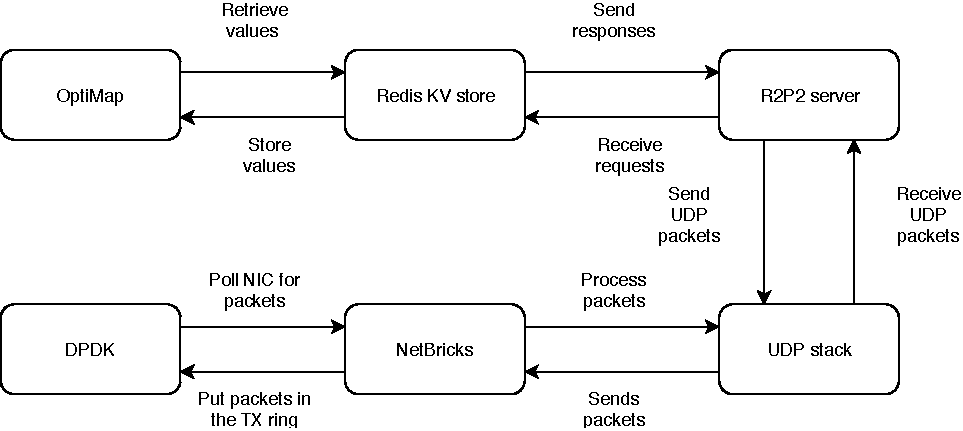
\includegraphics[width=\textwidth]{../diagram/overview.pdf}
  \caption{System overview}
  \label{fig:design-overview}
\end{figure}

Each packet is first received by DPDK from the NIC\@. The packets are
then processed through the NetBricks \marios{you just introduced NetBricks here. You should do that in the background as an example of a kernel bypassed system that you will later use.} pipeline to be handed over to the
UDP stack. The UDP stack then filters and matches packets to a given
socket. Each socket has an associated callback registered by the
user. In our case, the socket are created by the R2P2 server which
uses them to receive R2P2 requests from the network. Once every packet
in a request has been received, the R2P2 server then invokes its own
user callback, this time called the Request Callback. This callback
is registered by the last layer in the system, the actual key-value
store. The key-value store uses R2P2 to satisfy requests in the Redis
protocol. This is also where our hashmap comes in (though it is used
all across the system), to store the key value pairs.

\section{OptiMap} \label{sec:optimap-impl}

OptiMap is the name for the highly concurrent hashmap, described in
section~\ref{sec:local-store-design}, and we now will see how exactly
the design translates into a concrete Rust implementation.

\subsection{AtomicBox}

As stated in section~\ref{sec:local-store-design}, we need some way to
atomically swap values while also atomically reference counting them.
Unfortunately the rust standard library only provides a mean to
atomically swap raw pointers using the \textbf{AtomicPtr}
construct. This effectively forces us to make use of raw pointers,
thus not benefiting from any of Rust's memory safety guarantee and
potentially leading to memory corruption or leaks. Even though we are
forced to use unsafe, Rust still provides strong safety guarantees and
debugging time is still very much reduced since we know for sure that
memory corruption problems are located inside \textbf{unsafe} code
blocks.

\begin{figure}[htb!]
  \lstinputlisting{../code/abox.rs}
  \caption{The AtomicBox structure}
\end{figure}

This leads us to the \textbf{AtomicBox} abstraction, a safe wrapper
around \textbf{AtomicPtr}, that we will use to build our OMVCC
hashmap. The AtomicBox makes use of X86 CAS instructions to improve on
Arc. Arc provides an atomic reference count and AtomicBox provides an
atomic reference count as well the possibility to atomically swap that
value. Since every value is atomically reference counted it will stay
allocated as long as any reference to it still exists while allowing
new requests to fetch the newer value to do their work. Updates are
made using the value atomically fetched at that point in time,
creating a copy, modifying it as appropriate and then swapping it back
with the old one. If the swap succeeds the old value's reference count
is decreased (and dropped if we had the last reference), effectively
providing an optimistic multi-version concurrency control. If the swap
fails, i.e.\ someone already swapped it with another value, we repeat
the same process until the swap is successful.

To build the AtomicBox abstraction we make use of the capability of
Arc to be transformed into raw pointers, thus allowing a user to
control exactly how long the memory on the heap lives, including the
value outliving the AtomicBox instance. The reference can then be
transformed back into an Arc, although this requires using
\textbf{unsafe} since we turn arbitrary pointers into Arc instances
therefore introducing a risk of double-free or invalid memory
accesses.

\begin{figure}[htb!]
  \label{code:atomicbox-interface}
  \lstinputlisting{../code/abox_take.rs}
  \caption{AtomicBox public interface}
\end{figure}

The AtomicBox abstraction allows us to implement the optimistic
multi-version concurrency control scheme. Indeed, the AtomicBox allows
users to extract an Arc to the value referenced by the AtomicPtr it
contains. We can thus extract values from the AtomicBox and keep them
even when they are removed from the AtomicPtr as shown in
figure~\ref{code:atomicbox-interface}.

The public interface provided by AtomicBox aims to be simple, fast and
safe, hiding the unsafe details of the actual operation. We therefore
provide an idiomatic way to update the value as well as a clean way to
fetch the value. Updates are handled through closures, the user passes
a closure to the AtomicBox which will apply this closure to the
current value and then atomically replace the old value with the new
one. In order to allow the value contained in the AtomicBox to outlive
it, when getting the value we actually provide an Arc<T> to the user
making the allocation of the value itself independent from the
allocation of the AtomicBox.

Since they are to be shared amongst threads, all the hashmap
components are allocated on the heap, thus justifying our use of
Arcs. As all elements are of small size (most of them are one or two
pointers big), we make the claim that memory fragmentation is not
gonna be an issue in our case. Indeed most of the allocation with
respect to size will be coming directly from DPDK allocating memory
buffers from Linux's \textbf{hugepages} and thus won't affect the
heap.

\todo{Explain how the hashmap is built on top of AtomicBox}

\section{Networking}

Let's now dive into the networking layer of the system starting with
the lower layer, that is the interfacing with DPDK.

\subsection{DPDK} \todo{rephrase section}
\marios{First baragraph goes in the background.}
As you probably know, DPDK is a kernel-bypass networking framework
developed by Intel, typically for high-performance networking
applications. We thus implement all our networking stack on top of
DPDK. It provides drivers for Intel NICs and high-performance packet
management and allocation, as well as lots of networking related
libraries.

DPDK being written in C, we must first find some (ideally, convenient)
bindings allowing us to make calls into DPDK from Rust code. Another
thing to consider is the inherent unsafety in calling C code from
Rust. Since C code has none of the guarantees of Rust calls to C
functions must be in an unsafe block. A convenient safe Rust interface
is therefore a must for speed and ease of development.


\subsection{NetBricks}
\marios{Same here. Move the first paragraph in the background section 2 and talk only about the modifications here.}

\begin{figure}[htb!]
\begin{lstlisting}
ReceiveBatch::new(queue.clone())
    .parse::<MacHeader>()
    .parse::<IpHeader>()
    .metadata(box move |pkt|{
        // keep the source ip around for later replies
        pkt.get_header().src()
    })
    .parse::<UdpHeader>()
    .map(box move |pkt| {
        let src_addr = Ipv4Addr::from(*pkt.read_metadata());
        let src_port = pkt.get_header().dst_port();

        stack.sockets.get(&src_port).map(|sock| {
             sock.deliver(&pkt, src_addr, src_port)
        });
    })
    .compose()
\end{lstlisting}

  \label{code:udp-pipeline}
  \caption{UDP packet pipeline}
\end{figure}

In order to adapt NetBricks to end-host networking, the fork comes
with a few modifications in packet management. The first one is the
inability of packets to cross thread boundaries. Indeed since
NetBricks is geared towards network functions the packets are only
meant to be processed by the user defined pipeline and be freed as
soon as they have gone through the pipeline. To remedy this we create
the CrossPacket abstraction which can be created from the standard
NetBricks Packet and is able to cross thread boundaries by being
immutable. But we still need to be able to send packets through
NetBricks and NetBricks does not know how to handle CrossPackets. It
is therefore possible to convert a CrossPacket to a Packet as well as
the reverse.

\begin{figure}[htb!]
  \lstinputlisting{../code/cp.rs}
  \caption{CrossPacket abstraction}
  \label{code:crosspacket}
\end{figure}

The CrossPacket abstraction is the way we work within the limits of
the Rust type system. NetBricks' \textbf{Packet}s are, by default,
mutable meaning the Rust compiler will not allow them to cross thread
boundaries in order to prevent data races. However since the
pointer to the mbuf is immutable this poses a problem when sending the
packet. Indeed DPDK stores headers in the same buffer as the payload,
meaning we can't easily send the same payload concurrently to two
different destination. The way to solve this is make use of DPDK's
mbuf chaining, the first mbuf in the chain being local to the current
thread (therefore being mutable) and the second one being the
immutable payload shared between threads. This is the second notable
modification we make to our NetBricks fork, the ability to chain mbufs
to maintain the immutability of the packets we received from the
network while also having the possibility to send them concurrently to
different destinations.

One more thing that needs to be implemented in NetBricks is packets
living longer than the packet processing pipeline. Since NetBricks is
aimed at network function once a packet has gone through the packet
processing pipeline it has no reason to stay allocated (as in the case
of a firewall, when the decision has been made to forward the packet
it's not needed anymore). But in our case packets are longer lived, we
need to keep them in the store to answer queries later on. We then
need a way to prevent deallocation of packets once they leave the
pipeline. We make use of mbuf reference counts to do this. In our
segmented packets the headers always have a reference count of one,
indeed they are not needed once the packet has been sent successfully,
thus we let DPDK free them once the packet have gone through the
NIC\@. The payload on the other hand should not be deallocated after
sending, so we set its reference count to 2, thereby preventing DPDK
from freeing it. But we still need to free them once they are not
needed anymore. The problem here is that mbuf reference counts are not
atomic, this is a problem in our case since the same payload could be
sent from two different threads which will both need to increment
it. That means we need to wrap the actual payload and provide an
atomic reference counting capability to prevent mbufs from beeing
freed too early.

\subsection{UDP stack}

The UDP stack ties in to NetBricks by registering a pipeline on all
available cores and using each pipeline to dispatch packets to the
correct socket. Each socket is stored in a hashmap in the stack by its
port. Upon receiving a packet the stack filters in multiple steps the
packets dropping invalid ones and routing the others to the correct
socket. The corresponding callback is then called on the packets one
by one.

\begin{figure}[htb!]
  \lstinputlisting{../code/udp-sock.rs}
  \label{code:socket-registration}
  \caption{UDP stack public interface}
\end{figure}

The bind method shown in figure~\ref{code:socket-registration} allows
users to bind socket on a given UdpStack. The user provides the IP
address to listen on as well as the UDP port. In order to receive
incoming packets the user also provides a closure that will be called
every time a packet is read from the NIC by the UdpStack. The stack
will actually transfer ownership of the packets received to the
callback, thereby permitting the zero copy networking stack we are
aiming for.

The send method on the other hand does not need to transfer ownership
of the packets to the UDP stack, because it does not need to keep the
packets after sending them. Therefore it only borrows the Packet the
user wants to send. After which it creates a segmented DPDK packet to
allow sending the same packet concurrently to different destinations.
To avoid flooding the same RX ring, send() uses a simple round-robin
approach to select the output queue.

\subsection{R2P2 server} \todo{rephrase section}

We use a variant of the R2P2 protocol that adds active acknowledgement
from clients in order to reduce latency when packets are dropped. For
the sake of simplicity we also do not handle packets that are
delivered out of order, mostly to avoid resizing buffers used to store
the request while it is not completely received.

The R2P2 stack is built on top of the aforementioned UDP stack. The
R2P2 server registers a packet callback and then dispatches the packet
to the correct request after parsing the headers. Again the R2P2
server uses callbacks registered by the user application to handle
requests. These callbacks return a R2P2Response structure that is then
sent by the R2P2 server through the UDP stack.

The R2P2 server handles reliable delivery through client
acknowledgement. The response returned by the user callback is stored
in the R2P2 server while waiting for the acknowledgement and
retransmitted if need be.

\subsection{Key value store}

The key-value store uses a simplified version of the Redis
protocol. It only supports SET and GET requests, since the test
workload has no other type of requests.

\todo{Describe how we build keys and values from the raw Packets}

It then handles construction of the actual value that will be stored
in the hashmap. The requirements for the actual hashmap value and key
datastructures are mostly to play nice with the Rust memory management
model and DPDK mbufs. Indeed since we use segmented packets, we need
the headers to be freed once the request has been satisfied but the
payload itself must be kept as long as either the hashmap or the
networking hold it. As the payload can be sent concurrently from
different threads we need some sort of atomic reference counting on
the mbufs. The problem here is that mbufs reference counts are not
atomic (they're plain 16 bits integer).

%%% Local Variables:
%%% mode: latex
%%% TeX-master: "master"
%%% End:
